\documentclass{src/RPI-SIW}

% Load any necessary packages here
\usepackage[OT1]{fontenc}
\usepackage{graphicx,xcolor}
\usepackage{lipsum}
\usepackage{amsmath}
\usepackage{amsfonts}
\usepackage{amssymb}
\usepackage{float}

% Author and affiliation declaration
\author{
	% Author 1
	Chris R. Gnam\textsuperscript{1}\textsuperscript{*}
	and 
	% Author 2
	Andrew J. Liounis\textsuperscript{2},
    Coralie Adam\textsuperscript{3},
    Jason Leonard\textsuperscript{3},
    Peter Antreasian\textsuperscript{3},
    Dante S. Lauretta\textsuperscript{3},
    and the OSIRIS-REx Team;
	% First affiliation
	\textsuperscript{1}University at Buffalo, Department of Mechanical and Aerospace Engineering, 240 Bell Hall, Buffalo, NY  14260-4400
	% Second affiliation
	\textsuperscript{2}Goddard Space Flight Center, 8800 Greenbelt Rd, Greenbelt, MD 20771
    \textsuperscript{3}KinetX Space Flight Dynamics Practice, 21 West Easy Street, Simi Valley, CA 93065
    \textsuperscript{4}Lunar and Planetary Laboratory, University of Arizona, 1415 N 6th Ave, Tucson, AZ 85705
	% Email for POC (currently the first author)
	\textsuperscript{*}crgnam@buffalo.edu
}

% Title (it will be forced to all caps)
\title{A Novel Surface Feature Navigation Algorithm using Ray Tracing}

% Event title for the bottom left footer
\event{2\textsuperscript{nd} RPI Space Imaging Workshop. Saratoga Springs, NY. \\ 28-30 October 2019}


\begin{document}
% Build the custom title from the class file
\maketitle

% Custom abstract environment
\MakeAbstract{
    We demonstrate a novel single-pass ray tracing based approach to landmark identification for surface feature based relative navigation.  A priori knowledge of the camera pose and known topographic maps for each landmark are used to render the potentially visible landmarks via ray tracing into the image frame.  These templates are registered with a search region around the predicted location for each landmark in the image to estimate the observed landmark's position.  This procedure is applied to images from the Orbital A phase of the OSIRIS-REx mission, and the results are compared with those obtained via previous landmark identification methods.
}

\section*{Introduction}
The use of optical navigation (OpNav) for landmark tracking is critical for successful operations around small bodies.  Traditional radiometric tracking methods using the Deep Space Network (DSN) cannot provide the relative accuracy required to operate in close proximity these objects.  In these scenarios, OpNav can be used to directly relate the spacecraft state to the target surface.  The use of landmark-based surface feature navigation has been used to great success in missions such as Hayabusa\cite{hayabusa} and Rosetta\cite{rosetta}, which visited the asteroid Itokawa and the comet 67P, respectively.

As more ambitious small body exploration missions are conducted, landmark-based surface feature navigation must continue to improve.  Dr. Robert Gaskell's stereophotoclinometry (SPC) program is the current state-of-the-art, and has been used in a wide range of small body missions.  The performance of SPC has been studied extensively\cite{spc_sensitiviy}; however, there are some limitations in its methodology.

We propose a novel algorithm for landmark identification which can overcome many of the limitations faced by SPC.  In this paper we will explore the details of our new implementation, and compare its performance with SPC through a variety of methods.  We will also demonstrate the operational performance of this new methodology using navigation images from the OSIRIS-REx mission.

\section*{Review}
Gaskell's SPC software has been used for surface mapping and shape model reconstruction, as well as for landmark identification.\cite{gaskell2008} 

SPC's landmark identification functionality works by first predicting the expected locations of potentially visible landmarks using \textit{a priori} state knowledge of the spacecraft and pre-constructed landmark topographic maps, or \textit{maplets}.  The maplet topography is then illuminated using a Bidirectional Reflectance Distribution Function (BRDF), to create a \textit{predicted image}.  Next, the brightness values for all image points where a landmark is expected are extracted and projected onto the maplet surface, creating an \textit{extracted image}.  This represents what would be seen by looking directly down on the maplet.  Correlation based registration is then performed to align the extracted image and the predicted image.  Once all the predicted landmarks are found, a Perspective-n-Point (PnP) solver is run to adjust the camera pose, and the process can be repeated with improved accuracy.\cite{gaskell2011}

\begin{figure}[H]
	\centering
	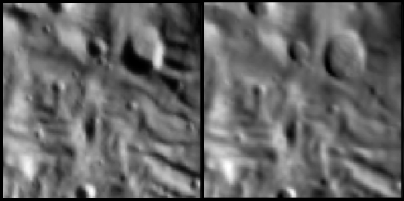
\includegraphics[width=0.4\textwidth]{figs/spc_sample.png}
	\caption{\textbf{Left:} Extracted image generated from brightness values in image projected onto maplet surface, \textbf{Right:} Predicted image generated from maplet and BRDF-based illumination}
	\label{figs::spc_match}
\end{figure}

There are several weaknesses associated with this method, however.  First, only the slope of the terrain is considered for illuminating the maplet.  This does not capture shadows in the scene, which are valuable pieces of information.  (The lack of shadows is clear in the predicted image in Fig. \ref{figs::spc_match}).  

In addition, because the image brightness data is extracted onto the surface, additional information about the maplet is artificially injected into the correlation that was not present in the original image.  This makes it possible to overfit the data, particularly when the landmarks are low resolution.

\section*{Proposed Methodology}
We propose a novel algorithm, which aims to solve both of these problems by utilizing a single-pass ray tracer.  This allows for the valuable shadow data to be properly traced, while also rendering the maplet into the image space where the correlation is then performed.  This algorithm can be broken into several primary steps.

\subsection*{Landmark Prediction}
Potentially visible features are identified using an \textit{a priori} estimate of the camera pose as well as the orientation of the target object. Once these potentially visible landmarks have been identified, they are projected into the camera frame (using a pre-calibrated camera model) to obtain the predicted centers for each.  

\subsection*{Template Rendering}
The topography data for all identified features are then loaded from a feature catalog.  Single-pass ray tracing is performed by tracing a set of rays (representing the pixels of the image), through a pre-calibrated model of the camera and identifying where they intersect with the maplet surface.  The rays are then traced back to the Sun, and any additional intersections indicate that the point on the maplet is in shadow.  This process identifies which rays intersected the surface, as well as the surface normal, incidence angle, and albedo for each intersection.  This information can then be run through a wide arrange of illumination models to fully render the illuminated surface into the image space, as a \textit{template}.


\subsection*{Cropping, Masking and Correlation}
Using the predicted centers for each landmark, a search region is defined around where the landmark is expected to be in the image.  The previously rendered templates are then registered with this search region to estimate where the landmark is in the region, and thus its location in the image as a whole.  The registration is done using a normalized correlation, and a least-squares algorithm is used to fit a paraboloid to the correlation surface.  This allows for sub-pixel accuracy in estimating the peak of the correlation surface, which corresponds to the estimated center of the landmark in the search region.

\subsection*{PnP and Measurement Refinement}
Once all landmark locations have been identified in the image, a PnP solver can be run to adjust the camera pose.  The templates are then re-rendered, and the image registration process is repeated with the new templates.  This allows for a more precise landmark location to be estimated.

\begin{figure}[h]
	\centering
	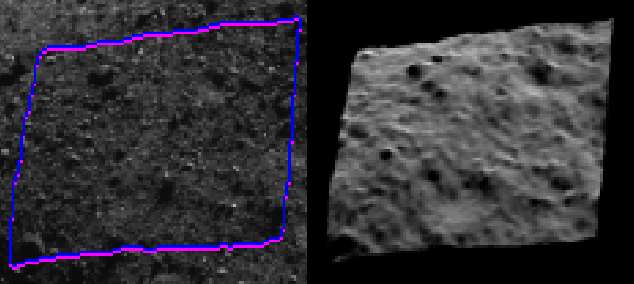
\includegraphics[width=0.4\textwidth]{figs/sfn_sample.png}
	\caption{\textbf{Left:} Cropped portion of NavCam image of Bennu in Orbital A, \textbf{Right:} Template of rendered maplet.  (Pink outline is the predicted location, blue outline is the solved-for location)}
	\label{figs::samplefit}
\end{figure}


\section*{OSIRIS-REx Orbital A}
The OSIRIS-REx asteroid sample return mission began proximity operations around near-Earth asteroid Bennu in December of 2018.  From January 2019 until March 2019, OSIRIS-REx was in the Orbital A mission phase, where it operated in a frozen terminator orbit around Bennu at altitudes roughly between 1.35km and 1.85km.  It was during this period of time that the navigation team transitioned from centroid-based relative navigation, to landmark-based navigation using SPC.

The method presented here was implemented into the Goddard Image Analysis and Navigation Tool (GIANT)\cite{andrew}, as the Surface Feature Navigation (SFN) module.  The GIANT SFN functionality was then used to process the navigation images from the Orbital A phase.  These results were then used along with radiometric measurements from the Deep Space Network (DSN) in the GEODYN II precision OD and geodetic parameter estimation program, to perform orbit determination.  The solutions obtained via this process were then compared with the trajectory solutions obtained by KinetX, the prime navigation team. 

\section*{Conclusions}
The results from the Orbital A processing showed extremely similar performance to SPC, the current state-of-the-art approach.  The final estimated trajectories differed by less than a meter throughout the entire observation period used.  This is a promising indication that continued development of this new approach will provide improved capabilities for future small body exploration missions.  Development and analysis will continue using navigation images from the OSIRIS-REx mission.

% All reference details are below.  Bibtex entries are in bib.bib
\vspace{3pt}
\bibliographystyle{src/ieeetr}
\titleformat{\section}[runin]{\normalsize\bfseries}{\thesection}{0em}{\addperiod}
{\footnotesize \bibliography{src/bib}}

\end{document}
